\documentclass[border=2mm]{standalone}

\usepackage{fontspec}
\usepackage{unicode-math}

\usepackage{pgfplots}
\pgfplotsset{compat=1.18}
\usetikzlibrary{arrows.meta, 
  calc, 
  positioning, 
  decorations.pathreplacing, 
  calligraphy}

\usepackage{xcolor}
\definecolor{den-1}{HTML}{111111}   % Đen #111111
\definecolor{den-2}{HTML}{222222}   % Đen #222222
\definecolor{den-3}{HTML}{333333}   % Đen #333333
\definecolor{den-4}{HTML}{444444}   % Đen #444444
\definecolor{den-5}{HTML}{555555}   % Đen #555555
\definecolor{den-6}{HTML}{666666}   % Đen #666666

% Thiết lập vị trí đặt nhãn gốc tọa độ
\tikzset{
  >=Stealth,
  originlabel/.style={
    font=\small\sf,
    anchor=north east, % Vị trí tương đối so với gốc
    yshift=-0.1ex,     % Điều chỉnh vị trí dọc một chút
    xshift=-0.1ex      % Điều chỉnh vị trí ngang một chút
  }
}

\begin{document}

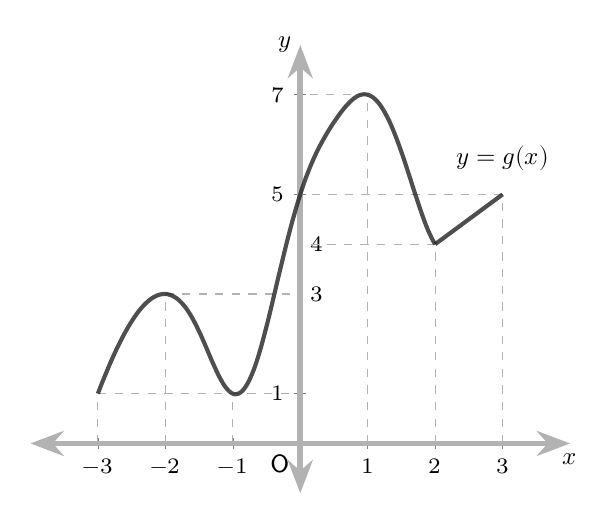
\begin{tikzpicture}

\begin{axis}[
    font=\small\sf,
    axis lines=middle,
    axis line style={<->, line width=2pt, color=den-6!50},
    xlabel=$x$, ylabel=$y$,
    xlabel style={below, font=\small\sf},
    ylabel style={left, font=\small\sf},
    xmin=-4, xmax=4,
    ymin=-1, ymax=8,
    xtick={-3 , -2 , -1 , 1 , 2 , 3},
    ytick={1 , 5 , 7},
    tick label style={font=\footnotesize\sf},
    clip=false,
]

\node[originlabel] at (axis cs:0,0) {O};

\node at (axis cs:0,3) [anchor=west] {\footnotesize $3$};

\node at (axis cs:0,4) [anchor=west] {\footnotesize $4$};


\draw [dashed, color=den-6!50] (-3,0) -- (-3,1) -- (0,1);
\draw [dashed, color=den-6!50] (-2,0) -- (-2,3) -- (0,3);
\draw [dashed, color=den-6!50] (-1,0) -- (-1,1);
\draw [dashed, color=den-6!50] (1,0) -- (1,7) -- (0,7);
\draw [dashed, color=den-6!50] (2,0) -- (2,4) -- (0,4);
\draw [dashed, color=den-6!50] (3,0) -- (3,5) -- (0,5);

\node at (3,5) [anchor=south, yshift=5] {$y=g(x)$};


\addplot[smooth, line width=1.5pt, color=den-2, opacity=.8] coordinates {
  (-3.000, 1.000)
  (-2.975, 1.089)
  (-2.950, 1.176)
  (-2.925, 1.262)
  (-2.899, 1.346)
  (-2.874, 1.429)
  (-2.849, 1.510)
  (-2.824, 1.590)
  (-2.799, 1.668)
  (-2.774, 1.744)
  (-2.749, 1.818)
  (-2.724, 1.891)
  (-2.698, 1.961)
  (-2.673, 2.030)
  (-2.648, 2.097)
  (-2.623, 2.162)
  (-2.598, 2.225)
  (-2.573, 2.286)
  (-2.548, 2.344)
  (-2.523, 2.401)
  (-2.497, 2.455)
  (-2.472, 2.507)
  (-2.447, 2.557)
  (-2.422, 2.605)
  (-2.397, 2.650)
  (-2.372, 2.692)
  (-2.347, 2.732)
  (-2.322, 2.770)
  (-2.296, 2.804)
  (-2.271, 2.837)
  (-2.246, 2.866)
  (-2.221, 2.893)
  (-2.196, 2.917)
  (-2.171, 2.938)
  (-2.146, 2.956)
  (-2.121, 2.971)
  (-2.095, 2.983)
  (-2.070, 2.992)
  (-2.045, 2.998)
  (-2.020, 3.000)
  (-1.995, 3.000)
  (-1.970, 2.996)
  (-1.945, 2.988)
  (-1.920, 2.977)
  (-1.894, 2.963)
  (-1.869, 2.945)
  (-1.844, 2.924)
  (-1.819, 2.899)
  (-1.794, 2.870)
  (-1.769, 2.837)
  (-1.744, 2.801)
  (-1.719, 2.760)
  (-1.693, 2.716)
  (-1.668, 2.667)
  (-1.643, 2.615)
  (-1.618, 2.559)
  (-1.593, 2.499)
  (-1.568, 2.436)
  (-1.543, 2.370)
  (-1.518, 2.300)
  (-1.492, 2.228)
  (-1.467, 2.153)
  (-1.442, 2.077)
  (-1.417, 1.999)
  (-1.392, 1.920)
  (-1.367, 1.840)
  (-1.342, 1.760)
  (-1.317, 1.680)
  (-1.291, 1.602)
  (-1.266, 1.526)
  (-1.241, 1.452)
  (-1.216, 1.381)
  (-1.191, 1.315)
  (-1.166, 1.253)
  (-1.141, 1.196)
  (-1.116, 1.145)
  (-1.090, 1.101)
  (-1.065, 1.063)
  (-1.040, 1.033)
  (-1.015, 1.010)
  (-0.990, 0.995)
  (-0.965, 0.988)
  (-0.940, 0.990)
  (-0.915, 1.001)
  (-0.889, 1.020)
  (-0.864, 1.048)
  (-0.839, 1.084)
  (-0.814, 1.130)
  (-0.789, 1.184)
  (-0.764, 1.247)
  (-0.739, 1.318)
  (-0.714, 1.397)
  (-0.688, 1.485)
  (-0.663, 1.579)
  (-0.638, 1.681)
  (-0.613, 1.790)
  (-0.588, 1.905)
  (-0.563, 2.026)
  (-0.538, 2.152)
  (-0.513, 2.283)
  (-0.487, 2.417)
  (-0.462, 2.555)
  (-0.437, 2.695)
  (-0.412, 2.837)
  (-0.387, 2.980)
  (-0.362, 3.124)
  (-0.337, 3.268)
  (-0.312, 3.411)
  (-0.286, 3.554)
  (-0.261, 3.695)
  (-0.236, 3.835)
  (-0.211, 3.972)
  (-0.186, 4.107)
  (-0.161, 4.238)
  (-0.136, 4.367)
  (-0.111, 4.493)
  (-0.085, 4.615)
  (-0.060, 4.733)
  (-0.035, 4.847)
  (-0.010, 4.957)
  (0.015, 5.063)
  (0.040, 5.165)
  (0.065, 5.263)
  (0.090, 5.357)
  (0.116, 5.447)
  (0.141, 5.533)
  (0.166, 5.615)
  (0.191, 5.693)
  (0.216, 5.768)
  (0.241, 5.840)
  (0.266, 5.909)
  (0.291, 5.975)
  (0.317, 6.039)
  (0.342, 6.101)
  (0.367, 6.160)
  (0.392, 6.218)
  (0.417, 6.275)
  (0.442, 6.329)
  (0.467, 6.383)
  (0.492, 6.435)
  (0.518, 6.485)
  (0.543, 6.534)
  (0.568, 6.582)
  (0.593, 6.628)
  (0.618, 6.673)
  (0.643, 6.715)
  (0.668, 6.756)
  (0.693, 6.795)
  (0.719, 6.831)
  (0.744, 6.865)
  (0.769, 6.896)
  (0.794, 6.924)
  (0.819, 6.948)
  (0.844, 6.969)
  (0.869, 6.985)
  (0.894, 6.998)
  (0.920, 7.006)
  (0.945, 7.009)
  (0.970, 7.008)
  (0.995, 7.002)
  (1.020, 6.991)
  (1.045, 6.975)
  (1.070, 6.954)
  (1.095, 6.927)
  (1.121, 6.896)
  (1.146, 6.860)
  (1.171, 6.818)
  (1.196, 6.771)
  (1.221, 6.719)
  (1.246, 6.663)
  (1.271, 6.601)
  (1.296, 6.535)
  (1.322, 6.464)
  (1.347, 6.389)
  (1.372, 6.310)
  (1.397, 6.227)
  (1.422, 6.140)
  (1.447, 6.050)
  (1.472, 5.956)
  (1.497, 5.860)
  (1.523, 5.761)
  (1.548, 5.660)
  (1.573, 5.557)
  (1.598, 5.453)
  (1.623, 5.348)
  (1.648, 5.242)
  (1.673, 5.136)
  (1.698, 5.031)
  (1.724, 4.926)
  (1.749, 4.823)
  (1.774, 4.722)
  (1.799, 4.623)
  (1.824, 4.528)
  (1.849, 4.436)
  (1.874, 4.348)
  (1.899, 4.266)
  (1.925, 4.189)
  (1.950, 4.119)
  (1.975, 4.055)
  (2.000, 4.000)
};


\addplot [smooth, line width=1.5pt, color=den-2, opacity=.8] coordinates {
  (2,4)
  (3,5)
};

\end{axis}

\end{tikzpicture}

\end{document}